\nnarticleheader{PID Control in Robotics}{Intel Chen '19}

At a very basic level, robotics can be seen as the process of intelligently controlling a motor or motors to complete a task. For example, controlling a robotic arm to grab an object. While robotic arms and many other applications of robotics involve movement in 3D space, they are in fact a combination of 1-dimensional movements. In the case of a 3D printer, where a printing nozzle moves in 3D space, the motion is usually accomplished by movements along linear rails in each of the X-, Y-, and Z-axes.

Robotics operations often require precise control of each of the robot’s axial movements. However, one cannot simply command the motors to go to the desired position. Actually, motors are only controlled by input voltage, which is proportional to the speed of the motor. The only commands that motors listen to are “faster” and “slower.” Sensors need to provide feedback to precisely control motors.

When a feedback loop is established, the sensor feeds information about the environment back to the motor so that the motor knows how to move. Then the new movement is again detected by the sensor and new feedback is generated. Because of this process, feedback loops are also called “close-loops.”

The simplest control is “bang-bang,” or the on-off method. This algorithm considers only whether the target is reached. When the current position is less than the target, the motor is set to +max; when the current position is greater than the target, the motor is set to -max. Using this control method, the robot should eventually approach the target, cross it, and then repeatedly cross back and forth, or oscillate. Due to the constant switching of motor direction, the robot usually makes a “bang-bang” noise, which has become the nickname for the method.

\[ \text{Output}_{\text{bang-bang}}(t) = \begin{cases}
    +\text{max}, & \text{for Input}(t) < \text{Target} \\
    -\text{max}, & \text{for Input}(t) > \text{Target} \\
    0, & \text{for Input}(t) = \text{Target}
\end{cases} \]

Since “bang-bang,” or the simple positive/negative determination of the error value, does not precisely lead the robot to the desired position, something more advanced is required. Implementing a PID controller is one of the ways to create a better close-loop control system. By definition, PID has a Proportional (P) component, Integral (I) component, and Derivative (D) component.

\[ e(t) \equiv \text{Input}(t) - \text{Target} \]
\[ \text{Output}_{\text{PID}}(t) = k_p * e(t) + k_i * \int_0^t{e(t)dt} + k_d * \frac{de(t)}{dt}|_{t=t} \]

The proportional component is the most significant and easy to understand. It takes the error—the difference between the desired position and the current position—and multiplies it by a kP constant. Thus, when the robot is far away from the desired position, the motor will run at a higher speed than when the robot is close to the desired position. Theoretically, a simple P-controller (controlled by only the P-component) would work perfectly. However, in reality, due to the delay in sensor feedback and processing, the P-controller often leads to minor oscillation like “bang-bang.” Also, the P-controller does not provide enough force when the error is too small—the motor prematurely stops before it reaches the target.

In the cases when the P-controller cannot bring the error to zero, the integral component becomes useful. It monitors the error over time through integration and adds to the motor voltage Ki*I. If the robot is stuck at a point for a period of time, the I-controller effectively learns that the motor needs to apply more force and help get the robot unstuck. In the context of competitive robotics, there can be foreign objects introduced into the path of the robot, so the I-component must be kept in a reasonable range to prevent motor values spiking to unsafe levels. Thus, the I-component is often limited by a maximum value.

The derivative component addresses the other problem with the P-controller: oscillation. The reason for the P-controller’s oscillation is overshooting caused by delay in sensor feedback. Before the sensor can tell the P-controller to stop, the robot often has already crossed the target and has to move backward. The derivative component can tell the robot to slow down when it is approaching the target too quickly.

\begin{figure}[H]
    \centering
    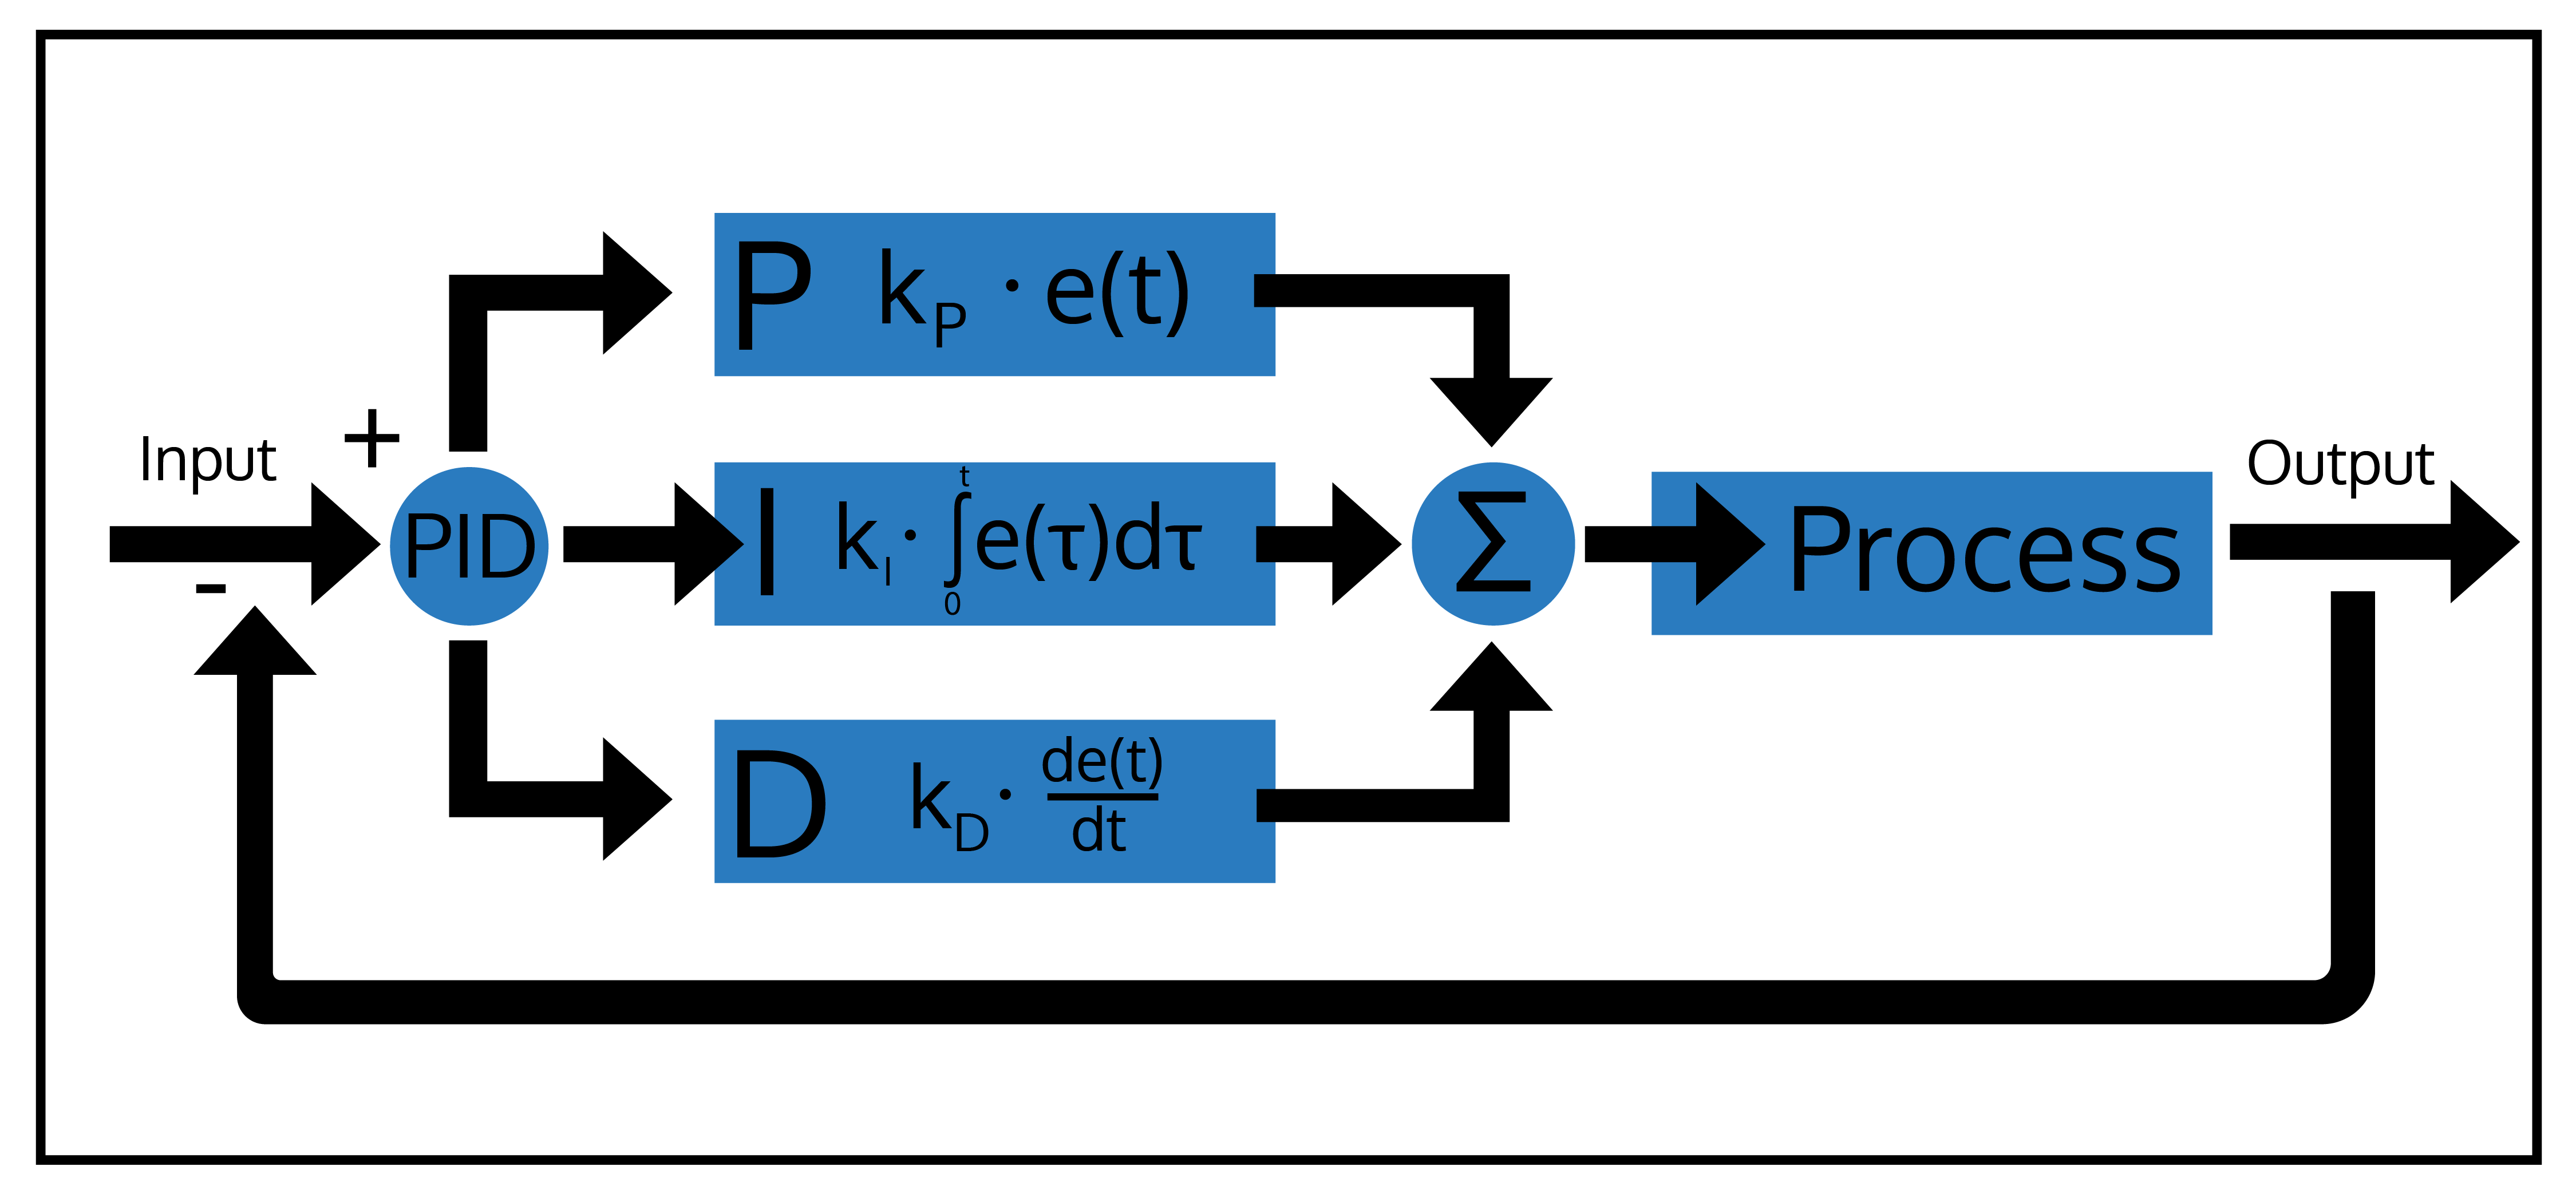
\includegraphics[scale=0.3]{assets/pid-graphic.png}
\end{figure}

When the three components are combined and the constants are properly tuned, PID controllers can greatly benefit the subsystems in robots. This increase in speed and accuracy translates directly into more accurate autonomous motion, leading to greater success.